%%%%%%%%%%%%%%%%%%%%%%%%%%%%%%%%%%%%%%%%%%%%%%%%%%%%%%%%%%%%
%2345678901234567890123456789012345678901234567890123456789012345678901234567890
%        1         2         3         4         5         6         7         8

%\documentclass[letterpaper, 10 pt, conference]{ieeeconf}  % Comment this line out
                                                          % if you need a4paper
\documentclass[a4paper, 10pt, conference]{ieeeconf}      % Use this line for a4
                                                          % paper

\IEEEoverridecommandlockouts                              % This command is only
                                                          % needed if you want to
                                                          % use the \thanks command
\overrideIEEEmargins
% See the \addtolength command later in the file to balance the column lengths
% on the last page of the document



% The following packages can be found on http:\\www.ctan.org
%\usepackage{graphics} % for pdf, bitmapped graphics files
%\usepackage{epsfig} % for postscript graphics files
%\usepackage{mathptmx} % assumes new font selection scheme installed
%\usepackage{times} % assumes new font selection scheme installed
%\usepackage{amsmath} % assumes amsmath package installed
%\usepackage{amssymb}  % assumes amsmath package installed
\usepackage{graphicx}
\usepackage{verbatim}
\usepackage{multirow}
\usepackage{rotating}
\usepackage{array}

\newcommand\T{\rule{0pt}{2.6ex}}
\newcommand\B{\rule[-1.2ex]{0pt}{0pt}}

\title{\LARGE \bf
An  Industrial Robotic Knowledge Representation for Kit Building Applications
}

\author{ \parbox{3 in}{\centering Stephen Balakirsky\\
         Intelligent Systems Division\\
         National Institute of Standards and Technology\\
        Gaithersburg, MD 20899, USA\\
         {\tt\small stephen.balakirsky@nist.gov}}
         \hspace*{ 0.5 in}
         \parbox{3 in}{ \centering Zeid Kootbally\\
          Department of Mechanical Engineering \\
         University of Maryland\\
         College Park, MD 20742, USA\\
         {\tt\small zeid.kootbally@nist.gov}}\\ \\
	\parbox{2.25 in}{\centering Craig Schlonoff\\
         Intelligent Systems Division\\
         National Institute of Standards and Technology\\
        Gaithersburg, MD 20899, USA\\
         {\tt\small craig.schlenoff@nist.gov}}
        \hspace*{0.05in}
         \parbox{2.25 in}{ \centering Thomas Kramer\\
          Department of Mechanical Engineering \\
         Catholic University of America\\
         Washington, DC 20064, USA\\
         {\tt\small thomas.kramer@nist.gov}}
        \hspace*{0.05in}
         \parbox{2.25 in}{ \centering Satyandra K. Gupta\\
          Maryland Robotics Center\\
         University of Maryland\\
         College Park, MD 20742, USA\\
         {\tt\small skgupta@umd.edu}}\\
}

%\author{Author1 and Author2% <-this % stops a space
%\thanks{This work was not supported by any organization}% <-this % stops a space
%\thanks{H. Kwakernaak is with Faculty of Electrical Engineering, Mathematics and Computer Science,
%        University of Twente, 7500 AE Enschede, The Netherlands
%        {\tt\small h.kwakernaak@autsubmit.com}}%
%\thanks{P. Misra is with the Department of Electrical Engineering, Wright State University,
%        Dayton, OH 45435, USA
%        {\tt\small pmisra@cs.wright.edu}}%
%}


\begin{document}



\maketitle
\thispagestyle{empty}
\pagestyle{empty}


%%%%%%%%%%%%%%%%%%%%%%%%%%%%%%%%%%%%%%%%%%%%%%%%%%%%%%%%%%%%
\begin{abstract}

The IEEE RAS Ontologies for Robotics and Automation Working Group is dedicated to developing a methodology for knowledge representation and reasoning in robotics and automation. As part of this working group, the Industrial Robots sub-group is tasked with studying industrial applications of the ontology. One of the first areas of interest for this subgroup is the area of kit building or kitting which is a process that brings parts together in a kit and then moves the kit to the assembly area where the parts are used in the final assembly. Kitting itself may be viewed as a specialization of the general bin-picking problem. This paper examines the knowledge representation that has been developed for the kitting problem and presents our implementation of the knowledge representation.

\end{abstract}


%%%%%%%%%%%%%%%%%%%%%%%%%%%%%%%%%%%%%%%%%%%%%%%%%%%%%%%%%%%%
\section{INTRODUCTION}
Kitting is the process in which several different, but related items are placed into a container and supplied together as a single unit.
In industrial assembly of manufactured products, kitting is often performed prior to final assembly. Manufacturers utilize kitting
due to its ability to provide cost savings \cite{Carlsson_2008} including saving manufacturing or assembly space \cite{Medbo2003}, reducing assembly workers walking and searching times \cite{Schwind1992}, and increasing line flexibility \cite{Bozer1992} and balance \cite{Jiao2000}.

Several different techniques are used to create kits. A kitting operation where a kit box is stationary until filled at a single
kitting workstation is refereed to as {\it batch kitting}. In {\it zone kitting}, the kit moves while being filled and will pass through one or
more zones before it is completed. This paper focuses on batch kitting processes.

In batch kitting, the kit's component parts may be staged in containers positioned in the workstation or may arrive on a conveyor.
Component parts may be fixtured, for example placed in compartments on trays, or may be in random orientations, for example
placed in a large bin. In addition to the kit's component parts, the workstation usually contains a storage area for empty kit boxes as
well as completed kits.

Kitting, has not yet been automated in many industries where automation may be feasible. Consequently, the cost of building kits is higher than it could be. We are addressing this problem by building models of the knowledge that will be required to operate an automated kitting workstation in an agile manufacturing environment. This workstation must be able to cope with
variations in kit contents, kit layout, and component supply. We also plan to develop a simulated kitting workstation for model validation. Our models
include representations for non-executable information about the workstation such as information about a robot, parts, kit designs, grippers, etc., models of executable information such as actions, preconditions, and effects, and models of the  process plan
necessary for kit construction. A discussion of the functional requirements for the process plan may be found in \cite{Balakirsky2012_1}.
For our automated kitting workstation, we assume that a robot performs a series of pick-and-place operations
in order to construct the kit. These operations include:
\begin{enumerate}
\item Pick empty kit and place on work table.
\item Pick multiple component parts and place in kit.
\item Pick completed kit and place in full kit storage area.
\end{enumerate}
Each of these actions may be a compound action that includes other actions such as end-of-arm tool changes, path planning,
and obstacle avoidance.

It should be noted that multiple kits may be built simultaneously. Finished kits are moved to the assembly floor where components
are picked
from the kit for use in the assembly procedure. The kits are normally designed to facilitate component picking in the correct
sequence for assembly. Component orientation may be constrained by the kit design in order to ease the pick-to-assembly process.
%The final kit does not normally contain small fasteners which are usually stored in the assembly area.
Empty kits are returned to the kit building area for reuse.

Although the knowledge requirements described in the previous paragraph have been identified for the kitting domain, they are clearly applicable to many types of industrial robot applications (and likely to robot applications in other fields). As such, we expect that these knowledge requirements will serve as the basis for the industrial robot ontology being developed in the IEEE  RAS Ontologies for Robotics and Automation Working Group \cite{Madhavan2011} (henceforth referred to as the IEEE WG). Throughout the process of developing the kitting ontology, the group will constantly look at the applicability of the requirements outside of kitting and move the pertinent knowledge ``up'' the ontology (whether in the portion that models the kitting sub-domain, the industrial robot domain, or the upper ontology), as appropriate.

In keeping with our philosophy of producing standards in conjunction with the IEEE WG, we wish the models being developed by this effort to be as widely applicable as possible. To support this desire,we have
created a layered model abstraction where users may adopt as many or few of the layers of the abstraction as make sense for their
specific application.  The architecture shown in Figure \ref{fig:ProcessDataFlow}, though developed for the implementation of the kitting ontology, can be equally applicable to the implementation of any type of formal manufacturing knowledge representation. Said in a different way, the implementor can plug in a knowledge representation for a different domain and the architecture would still be valid. In a similar manner, different planning language abstractions could be utilized in the middle-layer of the
abstraction and different planning/execution systems could be utilized in the top-layer of the abstraction.

Specifics on the overall architecture may be found in Section \ref{sect:Architecture}. An example of the
various knowledge representations and the flow from one to the next is presented in Section \ref{sect:Example}. Finally,
conclusions and future work may be found in Section \ref{sect:Conclusions}.

%%%%%%%%%%%%%%%%%%%%%%%%%%%%%%%%%%%%%%%%%%%%%%%%%%%%%%%%%%%%
\begin{figure}[htb]
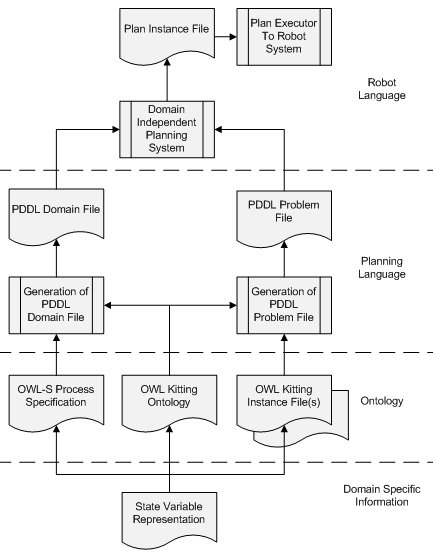
\includegraphics[width=8cm]{images/ProcessDataFlowV2.jpg}
\caption{Kitting data flow abstraction.}
\label{fig:ProcessDataFlow}
\end{figure}

\section{Architecture Description}
\label{sect:Architecture}
The main focus of this work is on the development of knowledge models that allow a kitting workstation to construct kits
in an agile manufacturing environment. However, in order to validate these knowledge models, we felt that it was
important to be able to utilize the models to construct kit building plans, and then to execute these plans in dynamic
virtual and real environments. Due to the advent of open source robotic operating systems such as ROS \cite{ROS}
 \footnote{Certain commercial software and tools are identified in this paper in order ot explain our research. Such identification does not imply
recommendation or endorsement by the authors, nor does it imply that the software tools identified are necessarily the best available for the purpose.}
 and simulation
packages such as USARSim \cite{Balakirsky2007} we do not need to design these systems ourselves. However, our architecture must
be designed to represent the required knowledge base in several different abstractions that are likely to be
required by these systems as the knowledge flows from domain and process specification, to plan generation, to plan execution.
As shown in Figure \ref{fig:ProcessDataFlow}, the abstraction is decomposed into four
distinct layers of {\it Domain Specific Information}, {\it Ontology}, {\it Planning Language}, and {\it Robot Language} that correspond to these
knowledge requirements. For the purposes of this paper, we will discuss the Domain Specific Information through Planning Language layers. Implementors of the abstraction are free to connect to the knowledge interface at the layer that makes sense for
their particular application. For our simulated kitting workstation, we intend to fully design the Domain Specific Information and the Ontology and
then utilize open
source tools that will automatically generate the remaining layers and provide a workstation simulation.

\subsection{Domain Specific Information}
\label{subsect:DomainSpecific}
The foundation for the knowledge representation is domain specific information that is produced by an expert in the particular field of study. This includes
information on items ranging from what actions and attributes are relevant, to what are the necessary conditions for an action to occur and what are the
likely results of that action. We have chosen to encode this basic information in a formalism know as a state variable representation (SVR) \cite{NAU.2004}.
This information will then flow up the abstraction and be transformed into the ontology, planning language, and robot language.
In a SVR, each state is represented by a tuple of values of $n$ state variables $\lbrace x_1,\dots,x_n\rbrace$, and each action is represented by a partial function that maps this tuple into some other tuple of values of the $n$ state variables. 

To build the SVR, the group has taken a very systematic approach of identifying and modeling the concepts. Because the industrial robot field is so broad, the group decided to limit its efforts to a single type of operation, namely kitting. A scenario was developed that described, in detail, the types of operations that would be performed in kitting, the sequencing of steps, the parts and machines that were needed, constraints on the process such as pre- and post-conditions, etc. For this scenario, a set of concepts were extracted and defined. These concepts served as the initial requirements for the kitting SVR. The concepts were then modeling in our SVR, building off of the definitions and relationships that were identified in the scenario.

A SVR relies on the elements of constant symbols, object variable symbols, state variable symbols, and planning operators. These are defined for the kitting domain in the rest of this section.

\subsubsection{Constant Symbols}
For the kitting domain, there is a finite set of constant symbols that must be represented in the system.
In the SVR, constant symbols are partitioned into disjoint classes corresponding to the objects of the domain. The finite set of all constant symbols in the kitting domain is partitioned into the following sets of constant symbols:
%\begin{small}
\begin{itemize}
\item A set of $\mathsf{Parts}$ $\lbrace\mathrm{p_1,p_2,\dots\rbrace}$: $\mathsf{Parts}$ are are the basic items that will be used to fill a kit.

\item A set of $\mathsf{PartTrays}$ $\lbrace\mathrm{pt_1,pt_2,\dots\rbrace}$: $\mathsf{Parts}$ arrive at the workstation in $\mathsf{PartTrays}$. Each part is at a known position in the $\mathsf{PartTray}$. Each $\mathsf{PartTray}$ contains one type of $\mathsf{Part}$.

\item A set of $\mathsf{KitTrays}$ $\lbrace\mathrm{kt_1, kt_2,\dots\rbrace}$:  A $\mathsf{KitTray}$ can hold $\mathsf{Parts}$ in known positions.

\item A set of $\mathsf{KitInstances}$ $\lbrace\mathrm{kins_1,kins_2,\dots\rbrace}$: A $\mathsf{KitInstance}$ is built when $\mathsf{Parts}$ are placed in a $\mathsf{KitTray}$. A $\mathsf{KitInstance}$ consists of a $\mathsf{KitTray}$ and, possibly, some $\mathsf{Parts}$. A $\mathsf{KitInstance}$ is empty when it does not contain any $\mathsf{Part}$ and finished when it contains all the $\mathsf{Parts}$ that constitute a kit.

\item A symbol $\mathsf{WorkTable}$ -- $\mathrm{wtable}$: A $\mathsf{WorkTable}$ is an area in the kitting workstation where $\mathsf{KitTrays}$ are placed to build $\mathsf{KitInstances}$.

\item A set of $\mathsf{LargeBoxWithKits}$ $\lbrace\mathrm{lbwk_1,lbwk_2,\dots\rbrace}$: A $\mathsf{LargeBoxWithKits}$ contains only finished $\mathsf{KitInstances}$.

\item A set of $\mathsf{LargeBoxWithEmptyKitTrays}$ $\lbrace\mathrm{lbwekt_1,lbwekt_2,\dots\rbrace}$: A $\mathsf{LargeBoxWithEmptyKitTrays}$ is a box that contains only empty $\mathsf{KitTrays}$.

\item A set of $\mathsf{Robots}$ $\lbrace\mathrm{r_1, r_2,\dots\rbrace}$: A $\mathsf{Robot}$ in the kitting workstation is a robotic arm that can move objects in order to build $\mathsf{KitInstances}$.

\item A set of $\mathsf{EndEffectors}$ $\lbrace\mathrm{eeff_1,eeff_2,\dots\rbrace}$: $\mathsf{EndEffectors}$ are used in a kitting workstation to manipulate $\mathsf{Parts}$, $\mathsf{PartTrays}$, $\mathsf{KitTrays}$, and $\mathsf{KitInstances}$. An $\mathsf{EndEffector}$ is attached to a $\mathsf{Robot}$.

\item A set of $\mathsf{EndEffectorHolders}$  $\lbrace\mathrm{eeffholder_1,eeffholder_2,\dots\rbrace}$: An $\mathsf{EndEffectorHolder}$ is a storage unit that holds one type of $\mathsf{EndEffector}$.

\item A symbol $\mathsf{EndEffectorChangingStation}$ -- $\mathrm{chstation}$: An $\mathsf{EndEffectorChangingStation}$ is made up of $\mathsf{EndEffectorHolders}$.
\end{itemize}
%\end {small}

\subsubsection{Object Variable Symbols}
Object variable symbols are typed variables which range over a class or the union of classes of constants. Examples of object variable symbols are $\mathrm{r}$ $\in$ $\mathrm{Robots}$, $\mathrm{kt}$ $\in$ $\mathrm{KitTrays}$, etc.

\subsubsection{State Variable Symbols}
A state variable symbol \emph{x}: $\mathrm{A_1\times \dots\times A_i}\times S\rightarrow\mathrm{B_1}$ $\cup$ $\dots$ $\cup$ $\mathrm{B_j}$ ($i, j\geq 1$) is a function from the set of states ($S$) and at least one set of constant variable symbols ($\mathrm{A_1\times \dots\times A_i}$) into a set of constant variable symbols ($\mathrm{B_1}$ $\cup$ $\dots$ $\cup$ $\mathrm{B_j}$). Using state variable symbols reduces the possibility of inconsistent states and generates a smaller state space. The following state variable symbols are used in the kitting domain:

%\begin{small}
\begin{itemize}
\item \emph{eEffLoc}: $\mathsf{EndEffectors}\times S\rightarrow\mathsf{Robots}$ $\cup$ $\mathsf{EndEffectorHolders}$: designates the location of an $\mathsf{EndEffector}$ in the workstation. The $\mathsf{EndEffector}$ can be placed in a $\mathsf{EndEffectorHolder}$ or attached to the $\mathsf{Robots}$.

\item \emph{rGrip}: $\mathsf{Robots}\times S\rightarrow\mathsf{EndEffectors}$ $\cup$ $\lbrace nil\rbrace$: designates the $\mathsf{EndEffector}$ that is attached to a $\mathsf{Robots}$ or $nil$ if no $\mathsf{EndEffector}$ is attached.

\item \emph{topWorkTable}: $\mathsf{WorkTable}\times S\rightarrow\mathsf{KitInstances}$ $\cup$ $\lbrace nil\rbrace$: designates the object placed on the $\mathsf{WorkTable}$, it can be either a $\mathsf{KitInstnce}$ or nothing ($nil$).

\item \emph{kInsLoc}: $\mathsf{KitInstances}\times S\rightarrow\mathsf{LargeBoxWithKits}$ $\cup$ $\mathsf{WorkTable}$ $\cup$ $\mathsf{Robots}$: designates the different possible locations of a $\mathsf{KitInstance}$ in the workstation. The $\mathsf{KitInstance}$ can be in a $\mathsf{LargeBoxWithKits}$, on the $\mathsf{WorkTable}$, or being held by the $\mathsf{Robot}$.

\item \emph{kTLoc}: $\mathsf{KitTrays}\times S\rightarrow\mathsf{LargeBoxWithEmptyKitTrays}$ $\cup$ $\mathsf{Robots}$: designates the different possible locations of a $\mathsf{KitTray}$ in the workstation. The $\mathsf{KitTray}$ can either be in a $\mathsf{LargeBoxWithEmptyKitTrays}$ or being held by the $\mathsf{Robot}$.

\item \emph{pLoc}: $\mathsf{Parts}\times S\rightarrow\mathsf{PartTrays}$ $\cup$ $\mathsf{KitInstances}$ $\cup$ $\mathsf{Robots}$: designates the different possible locations of a $\mathsf{Part}$ in the workstation. The $\mathsf{Part}$ can be in a $\mathsf{PartTray}$, in a $\mathsf{KitInstance}$, or being held by the $\mathsf{Robot}$.

\item \emph{rHold}: $\mathsf{Robots}\times S\rightarrow\mathsf{KitTrays}$ $\cup$ $\mathsf{KitInstances}$ $\cup$ $\mathsf{Parts}$ $\cup \lbrace nil\rbrace$: designates the object being held by the $\mathsf{Robots}$. It can be a $\mathsf{KitTray}$, a $\mathsf{KitInstance}$, $\mathsf{Part}$, or nothing ($nil$). It is assumed that the robot is already equipped with the appropriate $\mathsf{EndEffector}$.

\item \emph{isLBWKFull}: $\mathsf{LargeBoxWithKits}\times S\rightarrow \lbrace 0\rbrace \cup \lbrace 1\rbrace$: designates if a $\mathsf{LargeBoxWithKits}$ is full (1) or not (0).

\item \emph{isLBWEKTEmpty}: $\mathsf{LargeBoxWithEmptyKitTrays}\times S\rightarrow \lbrace 0\rbrace \cup \lbrace 1\rbrace$: designates if a $\mathsf{LargeBoxWithEmptyKitTrays}$ is empty (1) or not (0).

\item \emph{isPartTrayEmpty}: $\mathsf{PartTrays}\times S\rightarrow \lbrace 0\rbrace \cup \lbrace 1\rbrace$: designates if a $\mathsf{PartTray}$ is empty (1) or not (0).

\item \emph{eEffType}: $\mathsf{EndEffectors}\times S \rightarrow\mathsf{KitTrays}$ $\cup$ $\mathsf{Parts}$: designates the type of object the $\mathsf{EndEffector}$ can hold. For the kitting domain used in this paper, an $\mathsf{EndEffector}$ can hold two types of object: $\mathsf{KitTrays}$ and $\mathsf{Parts}$.
\end{itemize}
%\end{small}

\subsubsection{Planning Operators and Actions}
\label{subsect:Planning_Operators}
A planning operator~\cite{NAU.2004} is a triple \textit{o=(name(o), precond(o), effects(o))}
where:
\begin{itemize}
\item name(o) is a syntactic expression of the form $n(u_1,\dots,u_k)$, where $n$ is a symbol
called an operator symbol, $u_1,\dots,u_k$ are all of the object variable symbols that
appear anywhere in \textit{o}, and $n$ is unique (i.e., no two operators can have the
same operator symbol).
\item precond(o) is a set of expressions on state variables and relations.
\item effects(o) is a set of assignments of values to state variables of the form
$x(t_1,\dots,t_k)\leftarrow t_{k+1}$, where each $t_i$ is a term in the appropriate range.
\end{itemize}

The kitting domain is composed of eight operators. Only the operators' names and descriptions are mentioned in the rest of this section. Section~\ref{sect:Example} describes a more detailed operator through an example.

\begin{enumerate}
\item \textsl{take-kt} ($\mathrm{r}$, $\mathrm{kt}$, $\mathrm{lbwekt}$, $\mathrm{eeff}$): The $\mathrm{Robot}$ $\mathrm{r}$ equipped with the $\mathrm{EndEffector}$ $\mathrm{eeff}$ picks up the $\mathrm{KitTray}$ $\mathrm{kt}$ from the $\mathrm{LargeBoxWithEmptyKitTrays}$ $\mathrm{lbwekt}$.

\item \textsl{put-kt} ($\mathrm{r}$, $\mathrm{kt}$, $\mathrm{wtable}$): The $\mathrm{Robot}$ $\mathrm{r}$ puts down the $\mathrm{KitTray}$ $\mathrm{kt}$ on the $\mathrm{WorkTable}$ $\mathrm{wtable}$.

\item \textsl{take-kins} ($\mathrm{r}$, $\mathrm{kins}$, $\mathrm{wtable}$, $\mathrm{eeff}$): The $\mathrm{Robot}$ $\mathrm{r}$ equipped with the $\mathrm{EndEffector}$ $\mathrm{eeff}$ picks up the $\mathrm{KitInstance}$ $\mathrm{kins}$ from the $\mathrm{WorkTable}$ $\mathrm{wtable}$.

\item \textsl{put-kins} ($\mathrm{r}$, $\mathrm{kins}$, $\mathrm{lbwk}$): The $\mathrm{Robot}$ $\mathrm{r}$ puts down the $\mathrm{KitInstance}$ $\mathrm{kins}$ in the $\mathrm{LargeBoxWithKits}$ $\mathrm{lbwk}$.

\item \textsl{take-p} ($\mathrm{r}$, $\mathrm{p}$, $\mathrm{pt}$, $\mathrm{eeff}$): The $\mathrm{Robot}$ $\mathrm{r}$ uses the $\mathrm{EndEffector}$ $\mathrm{eeff}$ to pick up the $\mathrm{Part}$ $\mathrm{p}$ from the $\mathrm{PartTray}$ $\mathrm{pt}$.

\item \textsl{put-p} ($\mathrm{r}$, $\mathrm{p}$, $\mathrm{kins}$): The $\mathrm{Robot}$ $\mathrm{r}$ puts down the $\mathrm{Part}$ $\mathrm{p}$ in the $\mathrm{KitInstance}$ $\mathrm{kins}$.

\item \textsl{attach-eeff} ($\mathrm{r}$, $\mathrm{eeff}$, $\mathrm{eeffholder}$): The $\mathrm{Robot}$ $\mathrm{r}$ attaches the $\mathrm{EndEffector}$ $\mathrm{eeff}$ from the $\mathrm{EndEffectorHolder}$ $\mathrm{eeffholder}$.

\item \textsl{remove-eeff} ($\mathrm{r}$, $\mathrm{eeff}$, $\mathrm{eeffholder}$): The $\mathsf{Robot}$ $\mathrm{r}$ removes the $\mathrm{EndEffector}$ $\mathrm{eeff}$ and puts it in the $\mathrm{EndEffectorHolder}$ $\mathrm{eeffholder}$.
\end{enumerate}

An action \textit{a} can be obtained by substituting the object variable symbols that
appear anywhere in \textit{o} with constant symbols. For instance, the operator \textsl{take-p}($\mathrm{r}$, $\mathrm{p}$, $\mathrm{pt}$, $\mathrm{eeff}$) in the kitting domain can be translated into the action \textsl{take-p}($\mathrm{r_1}$, $\mathrm{p_1}$, $\mathrm{pt_1}$, $\mathrm{eeff_2}$) where $\mathrm{r_1}$, $\mathrm{p_1}$, $\mathrm{pt_1}$, and $\mathrm{eeff_2}$ are constant symbols in the classes $\mathsf{Robots}$, $\mathsf{Parts}$, $\mathsf{PartTrays}$, and $\mathsf{EndEffectors}$, respectively.
\subsection{Ontology}
``Ontology deals with questions concerning what entities exist or can be said to exist, and how such entities can be grouped, related within a hierarchy, and subdivided according to similarities and differences'' \cite{ontologyDef}.

Knowledge models may take many forms ranging from informal natural language, to XML schemas, to ontologies.
For the development of the  knowledge representation, the industrial robots sub-group has decided to use the  Web Ontology Language (OWL) \cite{OWL} as the knowledge representation language. OWL is a family of knowledge representation languages for authoring ontologies and is endorsed by the World Wide Web Consortium (W3C). It is characterized by formal semantics and Resource Description Framework/eXtensible Markup Language (RDF/XML)-based serialization for the Semantic Web. OWL was chosen by the group because of its popularity among the ontology development community, its endorsement by the W3C, as well as the number of tools and reasoning engines that are available. OWL was also selected as the representation language that will be used in the overall IEEE WG efforts.

In addition to OWL, the industrial robots subgroup will also be using OWL-S \cite{Martin2012} to represent the processes and actions that the robot will perform. OWL-S is an ontology built on top of OWL by the DARPA Agent Markup Language (DAML) program \cite{damlWeb}
for describing Semantic Web Services. However, many of the constructs that are used to describe services are equally applicable to encoding our SVR. For example, concepts such as preconditions, results, inputs, outputs, effects, and participants are generic enough to be applied to just about any type of process specification.

Since this work is being directed at the IEEE RAS Ontologies for Robotics and Automation Working Group, it is appropriate that our  domain specific knowledge  be
encoded in an OWL ontology at the first domain independent  layer of our abstraction. The knowledge contained in this layer is derived from our SVR and may also contain
information that has been collected over other domains. The knowledge is sufficient for a planning system to understand the specific problem domain and construct
a plan for creating the desired kit from the given resources.

As more detailed scenarios are determined and a richer set of concepts are uncovered, the ontology will be partitioned based upon the generality of the concept, with the most generally applicable concepts being ``higher'' in the ontology so they are available to other domains and the more detailed concepts being ``lower'' in the ontology because they will likely be very specific to the kitting area. An example of a general concept may be a $\mathrm{Robot}$ while a specific concept may be a $\mathrm{KitTray}$.

As shown in Figure \ref{fig:ProcessDataFlow}, the information in our ontology is divided into three files and consists of a representation of the process specification,
the kitting ontology, and the instance file. The process specification file is based off of the planning operators from the SVR and contains descriptions of
the individual actions and sequences necessary to construct a kit, e.g. gripping a component from a tray. The kitting ontology file is based off of the constant symbols and
state variable symbols and contains the concepts related to the specific items
that compose the kitting domain, e.g. the hierarchy of what it means to be a $\mathrm{Part_a}$. That a $\mathrm{Part_a}$ is a type of $\mathrm{Part}$, and that
all $\mathrm{Parts}$ contain properties such as the part's weight, dimensions, and grip points. The instance file is based off of the SVR object variable symbols and
contains specific information on {\it this} particular kitting problem and configuration, e.g. $\mathrm{KitTray kt_1}$ contains 4 $\mathrm{Parts}$ of type $\mathrm{Part_a}$.

While this file set provides a complete description of the problem domain and environment, most planning systems cannot directly ingest information from an ontology.
Therefore, the next layer of the data abstraction known as the Planning Language layer was created.

\subsection{Planning Language}
The Planning Domain Definition Language (PDDL) \cite{PDDL} is an attempt by the domain independent planning community to formulate a standard language for planning. A community
of planning researchers has been producing planning systems that comply with this formalism since the first International Planning Competition held in 1998. This competition series
continues today, with the seventh competition being held in 2011. PDDL is constantly adding extensions to the base language in order to represent more expressive problem domains. Our
work is based on PDDL Version  3.

By placing our knowledge in a PDDL representation, we enable the use of an entire family of open source planning systems.
As shown in Figure \ref{fig:ProcessDataFlow}, each PDDL file-set consists of two files that specify the domain and the problem. The PDDL domain file is composed of four sections that include
requirements, types and constants, predicates, and actions. This file may be automatically generated from a combination of information that is contained in the OWL-S process specification file and the OWL Kitting Ontology file. 

The requirements section specifies which extensions this problem domain relies on. The planning system can examine this statement to determine if it is capable of solving problems in this domain. In PDDL, all variables that are used in the domain must be typed. Types are defined in the $\mathrm{types}$ section. It is also possible to have constants that specify that all problems will share this single value. For example, in the simplest kitting workstation we will have a single $\mathrm{Robot}$ $\mathrm{r_1}$.
Predicates specify relationships between instances. For example, an instance of a $\mathrm{KitTray}$, $\mathrm{kt_1}$, can have a physical location and contains instances of $\mathrm{Parts}$, $\mathrm{Part_a}$, $\mathrm{Part_b}$, and $\mathrm{Part_c}$. The final section of the PDDL domain file is concerned with actions. An action statement specifies a way that a planner affects the state of the world. The statement includes parameters, preconditions, and effects. The preconditions dictate items that must be initially true for the action to be legal. The effect equation dictates the changes in the world that will occur due to the execution of the action.

The second file of the PDDL file-set is a  problem file. The problem file specifies information about the specific instance of the given problem. This file contains the initial conditions and definition of the world (in the init section) and the final state that the world must be brought to (in the goal section). A specific example of the ontology to planning language conversion is provided in Section \ref{sect:Example}.

%\subsection{Robot Plan Conformance}
%\label{subsect:RobotPlan}
%Any one of a number of open source planning systems may now be run on the Planning Language layer's knowledge representation. The output of these planners will be
%a PDDL action sequence file that is based on our original vocabulary. This file
%contains a time sequenced series of actions that must be carried out in order to create a transition from our initial system state to the goal system state. It should be noted that
%the sequence of knowledge transformations that takes place from the ontology through the planning language, to the action sequence is independent of the kitting domain or any specific %hardware configurations and is able to solve problems for many types of industrial robot applications.
%The top layer of our abstraction ties the specific commands to the kitting workstation and is dependent on the workstation's resident hardware.  In order to maintain as
%much hardware independence as possible, we have chosen to use the ROS environment for communicating with our simulation. Therefore, the PDDL commands will
%be translated into appropriate commands that will be sent into various ROS processes. These ROS stacks will then control all aspects of our USARSim virtual workstation.

%%%%%%%%%%%%%%%%%%%%%%%%%%%%%%%%%%%%%%%%%%%%%%%%%%%%%%%%%%%%
\section{Example of Operation}
\label{sect:Example}
The purpose of this section is to illustrate the various knowledge representations, depicted in Figure~\ref{fig:ProcessDataFlow}, and the flow from one knowledge representation to the next.

\subsection{State Variable Representation}

In the example, the \class{Robot} has to build a kit that contains two \class{Parts} of type A, one \class{Part} of type B and one \class{Part} of type C. The kitting process is completed once the kit is placed in the \class{LargeBoxWithKits}. Section \ref{subsect:PDDL_Domain_File} details the steps that build the PDDL domain file while Section~\ref{subsect:PDDL_Problem_File} discusses the process that builds the PDDL problem file.

The state variable representation defines the necessary parameters for the PDDL domain and problem files. The PDDL domain file contains predicates, characterized by state variable symbols, and actions. The PDDL problem file contains the objects present in the problem instance, characterized by constant variable symbols, the initial state $s_0$ description and the goal $s_G$.

\paragraph{Constant Variable Symbols}
The kitting domain proposed for the example contains a \class{Robot} \const{r_1}, a \class{KitTray} \const{kt_1}, a \class{LargeBoxWithEmptyKitTrays} \const{lbwekt_1}, a \class{LargeBoxWithKits} \const{lbwk_1}, a \class{WorkTable} \const{wtable}, three \class{PartTrays} \const{pt_{A}}, \const{pt_{B}}, and \const{pt_{C}}, \class{Parts} \const{part_{A-1}}, \const{part_{A-2}}, \const{part_{B}}, and \const{part_{C}}, two \class{EndEffectors} \const{eff_1} and \const{eff_2}, and two  \class{EndEffectorHolders} \const{effh_1} and \const{effh_2}. Since a \class{KitInstance} is by definition a \class{KitTray} that contains \class{Parts}, the kitting domain also contains a constant variable symbol \const{kins_1} from \class{KitInstance}.

\paragraph{State Variable Symbols}
The state variable symbols for the kitting domains are the ones defined in section \ref{subsubsect:State_Variable_Symbols}.

\paragraph{Rigid Relations}
\begin{comment}
As stated in section \ref{subsubsect:Rigid_Relation}, the kitting domain has two rigid relations: \stvar{efftype} and \stvar{effhtype}. In the proposed example, the \class{EndEffector} \const{eff_1} can hold \class{KitTrays} and \class{KitInstances}, while the \class{EndEffector} \const{eff_1} can hold \class{Parts}. \stvar{efftype} can be stated as follows: \stvar{efftype}(\const{eff_1})=\{\const{kt_1},\const{kins_1}\} and \stvar{efftype}(\const{eff_1})=\{\const{part_{A-1}},\const{part_{A-2}},\const{part_{B}},\const{part_{C}}\}. In the same way, the \class{EndEffectorHolder} \const{effh_1} can hold the \class{EndEffector} \const{eff_1}, while the \class{EndEffectorHolder} \const{effh_2} can hold the \class{EndEffector} \const{eff_2}. \stvar{effhtype} can be stated as follows: \stvar{effhtype}(\const{effh_1})=\{\const{eff_1}\} and \stvar{effhtype}(\const{effh_2})=\{\const{eff_2}\}.
\end{comment}
As stated in section \ref{subsubsect:Rigid_Relation}, the kitting domain has two rigid relations: \stvar{efftype} and \stvar{effhtype} that can be stated as follows: \stvar{efftype}(\const{eff_1})=\{\const{part_{A-1}},\const{part_{A-2}},\const{part_{B}},\const{part_{C}}\} and \stvar{efftype}(\const{eff_2})=\{\const{kt_1},\const{kins_1}\}. In the same way, \stvar{effhtype} can be stated as follows: \stvar{effhtype}(\const{effh_1})=\{\const{eff_1}\} and \stvar{effhtype}(\const{effh_2})=\{\const{eff_2}\}.

\paragraph{Initial State}
The initial state $s_0$ can be represented by the following set of state variable symbols:\\
$s_0$=\{\stvar{rhold}(\const{r_1})=\textit{nil}, \stvar{effloc}(\const{eff_1})=\const{effh_1}, \stvar{effloc}(\const{eff_2})=\const{effh_2}, \stvar{isptempty}(\const{pt_A})=0, \stvar{isptempty}(\const{pt_B})=0, \stvar{isptempty}(\const{pt_C})=0, \stvar{onworktable}(\const{wtable})=\textit{nil}, \stvar{islbwektempty}(\const{lbwekt_1})=0, \stvar{islbwkfull}(\const{lbwk_1})=0, \stvar{partloc}(\const{part_{A-1}})=\const{pt_A}, \stvar{partloc}(\const{part_{A-2}})=\const{pt_A}, \stvar{partloc}(\const{part_{B}})=\const{pt_B}, \stvar{partloc}(\const{part_{C}})=\const{pt_C}, \stvar{ktloc}(\const{kt_1})=\const{lbwekt_1}\}.

\begin{comment}
In the initial state $s_0$, the $\mathsf{Robot}$ $\mathrm{r_1}$ is not equipped with any $\mathsf{EndEffector}$ and is not holding anything. The $\mathsf{EndEffectors}$ $\mathrm{eeff_1}$ and $\mathrm{eeff_2}$ are placed in the $\mathsf{EndEffectorHolders}$ $\mathrm{eeffholder_1}$ and $\mathrm{eeffholder_2}$, respectively. The $\mathsf{LargeBoxWithKits}$ $\mathrm{lbwk_1}$ is not full. The $\mathsf{LargeBoxWithEmptyKitTrays}$ $\mathrm{lbwekt_1}$ is not empty. The $\mathsf{PartTrays}$ $\mathrm{pt_A}$, $\mathrm{pt_B}$, and $\mathrm{pt_C}$ are not empty. The $\mathsf{WorkTable}$ $\mathrm{wtable}$ is free of any object.
\end{comment}

\paragraph{Goal State}
\begin{comment}
The goal state $s_g$, the $\mathsf{KitInstance}$ $\mathrm{kins_1}$ contains $\mathsf{Parts}$ $\mathrm{p_{A-1}}$, $\mathrm{p_{A-2}}$, $\mathrm{p_{B-1}}$, and $\mathrm{p_{C-1}}$. The $\mathsf{KitInstance}$ $\mathrm{kins_1}$ is placed in the $\mathsf{LargeBoxWithKits}$ $\mathrm{lbwk_1}$.
\end{comment}
The goal state $s_G$ can be represented by the following set of state variable symbols:\\
$s_g$ =\{\stvar{partloc}(\const{part_{C}})=\const{kins_1}, \stvar{partloc}(\const{part_{B}})=\const{kins_1}, \stvar{partloc}(\const{part_{A-2}})=\const{kins_1}, \stvar{partloc}(\const{part_{A-1}})=\const{kins_1},   \stvar{kinsloc}(\const{kins_1})=\const{lbwk_1}\}.

\paragraph{Action}
Among the eight planning operators introduced in Section \ref{subsect:Planning_Operators}, only the planning operator \op{take-kt}(\const{r},\const{kt},\const{lbwekt},\const{eff}) will be discussed in this example. By substituting the object variable symbols described in the definition of the planning operator \op{take-kt} with the constant variable symbols defined in this example, the following action is produced:

\begin{itemize}
\item \op{take-kt}(\const{r_1},\const{kt_1},\const{lbwekt_1},\const{eff_2}): The \class{Robot} \const{r_1} equipped with the \class{EndEffector} \const{eff_2} picks up the \class{KitTray} \const{kt_1} from the \class{LargeBoxWithEmptyKitTrays} \const{lbwekt_1}.
\begin{itemize}
\item precond: \stvar{ktloc}(\const{kt_1})=\const{lbwekt_1}, \stvar{rhold}(\const{r_1})=\textit{nil}, \stvar{reff}(\const{r_1})=\const{eff_2}, \stvar{effloc}(\const{eff_1})=\const{r_1}, \stvar{islbwektempty}(\const{lbwekt_1})=0
\item effects: \stvar{ktloc}(\const{kt_1})$\leftarrow$\const{r_1}, \stvar{rhold}(\const{r_1})$\leftarrow$\const{kt_1}
\end{itemize}
\end{itemize}

\subsection{Process for the PDDL Domain File}
\label{subsect:PDDL_Domain_File}
Once the state variable representation is defined, an OWL-S process specification and OWL ontology is built. This must be constructed by hand from the information in the SVR as described in Section \ref{subsect:Ontology}. For this example, the specific action  \op{take-kt}'s encoding into OWL-S will be discussed.

\subsubsection{OWL-S Representation}
Once the action is specified in the SVR, we can use that information to create an OWL-S process. We are modeling the action as a process and including information about its data inputs and outputs, the preconditions that have to be true for it to be performed, and the result that will be true after the process is executed. In our example, the process is an atomic process because it only involves a single interaction and consists of only one step. If it were a more complex process that involved multiple sub-actions, it would be modeled by an OWL-S composite process.

In the SVR, the preconditions clearly map to the OWL-S preconditions. 
%These can be represented in languages such as KIF \cite{KIF} (Knowledge Interchange Format), SPARQL \cite{SPARQL} (SPARQL Protocol and RDF Query Language), or SWRL \cite{SWRL-W3C} (Semantic Web Rule Language). 
The rules point to classes and instances in the ontology that model the concepts of kit tray (\const{kt}), a set of large box with empty kit trays (\const{lbwekt}), a robot (\const{r}), and a robot end effector (\const{eff}). The SVR effects map to the OWL-S results and are also represented in one of the rules languages above. In the case of the \op{take-kt} action, the result would specify that the location of the kit tray is no longer in a fixed location and is now in the robot end effector.

Though not explicitly represented in the SVR, data inputs and outputs are an important part of the OWL-S representation and can be inferred from the SVR. Specifically, it needs to know which robot is performing the action (\const{r_1}), which kit tray needs to be picked up (\const{kt_1}), which end effector is on the robot (\const{eff_2}), and from which box the robot needs to pick up the kit tray (\const{lbwekt_1}). The output of this action would be a Boolean stating whether the action was completed successfully or not.

\begin{figure}[h!]
%\begin{center}
\centering
\begin{minipage}{.5\paperwidth}
\begin{mylisting}
\begin{Verbatim}[commandchars=\\\{\},commandchars=+\[\],fontsize=\scriptsize,numbersep=3pt]
(define (domain kitting-domain)
 (:requirements :strips :typing)
 (:types part parttray kittray kitinstance worktable
  largeboxwithkits largeboxwithemptykittrays robot
  endeffector ...)
 (:predicates
  (effloc ?eff - endeffector ?r - robot
   ?effh - endeffectorholder)
  (efftype ?effh - endeffectorholder ?eff - endeffector)
   ...  )
 (:action take-kt
  :parameters (?r - robot ?kt - kittray
   ?lbwekt - largeboxwithemptykittrays
   ?eff - endeffector)
  :precondition (and (rhold ?robot ?nil)
     (ktloc ?kittray ?largeboxwithemptykittrays)
     (reff ?robot ?endeffector)
     (effloc ?kittray ?robot)
     (not (islbwektempty (?largeboxwithemptykittrays))))
  :effect (and (ktloc ?kittray ?robot)
          (rhold ?robot ?kittray))  )
\end{Verbatim}
\end{mylisting}
\end{minipage}
\caption{Excerpt of the PDDL domain file for kitting.\label{fig:domainfile}}
%\end{center}
\vspace{-.15in}
\end{figure}

\subsubsection{PDDL Domain File}
An external tool is used to generate the PDDL Domain File from the OWL/OWL-S representation. Due to space constraints, only an excerpt of the PDDL domain file is displayed in Figure \ref{fig:domainfile}.

\subsection{Process for the PDDL Problem File}
\label{subsect:PDDL_Problem_File}
The PDDL problem file is generated by a chain of data conversions that take the SVR through an OWL representation to the PDDL representation.
\subsubsection{OWL Representation}
The OWL instance files shown in Figure \ref{fig:ProcessDataFlow} are derived from the SVR initial and goal states ($s_0$, $s_G$). These files contain
specific instances of the classes that have been previously defined in the OWL ontology. Two specific instance files are required for the representation with
both files containing the same class structures. The difference between the two is that in the \const{InitFile} the specific properties of the instantiated 
classes represent the initial state of the domain, and in the \const{GoalFile} the specific properties of the instantiated classes represent the goal state
of the domain.

\begin{figure}[h!]
%\begin{center}
\centering
\begin{minipage}{.5\paperwidth}
\begin{mylisting}
\begin{Verbatim}[commandchars=\\\{\},commandchars=+\[\],fontsize=\scriptsize,numbersep=3pt]
(define (problem kitting-problem)
 (:requirements :strips :typing)
 (:domain kitting-domain)
 (:objects r1 kt1 lbwekt1 lbwk1 wtable ptA ptB ptC
  partA-1 partA-2 partB partC eff1 eff2 effh1
  effh2 kins1)
 (:init  (rhold r1 nil) (effloc eff1 effh1)
  (effloc eff2 effh2) (not (isptempty ptA))
  (not (isptempty ptB)) (not (isptempty ptC))
  (onworktable wtable nil) (not (islbwektempty lbwekt1))
  (not (islbwkfull lbwk1)), (partloc partA-1 ptA)
  (partloc partA-2 ptA) (partloc partB ptB)
  (partloc partC ptC) (ktloc kt1 lbwekt1))
 (:goal (and (partloc partA-1 kins1)
  (partloc partA-2 kins1) (partloc partB kins1)
  (partloc partC kins1) (kinsloc kins1 lbwk1)))
\end{Verbatim}
\end{mylisting}
\end{minipage}
\caption{Excerpt of the PDDL problem file for kitting.\label{fig:problemfile}}
%\end{center}
\end{figure}

\subsubsection{PDDL Problem File}
The PDDL file is once again automatically generated. An excerpt of the PDDL problem file is shown in Figure \ref{fig:problemfile}. This file
contains the required sections of requirements, initial conditions, and goal conditions.

\subsubsection{PDDL File Processing}
Once the PDDL files have been generated, a wide variety of planners exist that could be used to generate a PDDL solution file. In our particular implementation, we are utilizing a variant of the classical FF system by Hoffmann and Nebel \cite{Hoffmann2001}.







%%%%%%%%%%%%%%%%%%%%%%%%%%%%%%%%%%%%%%%%%%%%%%%%%%%%%%%%%%%%
\section{CONCLUSIONS AND FUTURE WORK}
\label{sect:Conclusions}
In this paper we have presented the first knowledge model that is part of the IEEE RAS Ontologies for Robotics and Automation, Industrial Robotics subgroup on kitting.
This abstraction begins with data that has been created by an expert user as a state variable representation and encoded into an OWL ontology. The knowledge
is the automatically transitioned into a Planning Domain Definition Language that may be used by a class of planners to find a solution that will provide for actions that will
transition the system for its initial state to a prescribed goal state.

This workstation is still very much a work in progress. The IEEE working group has an active mailing list and meets in person at both the IEEE ICRA and IROS conferences.
At present, we are working on connecting the planned action sequence through the ROS control stack to our USARSim virtual world. As the knowledge representation is
exercised, it is expected that short comings and missing data will be detected. Our representation will be updated as necessary to cope with these developments. In addition,
the representation will be expanded to include metrics that allow us to represent not only the the information necessary for the construction of a kit, but also for the representation
of the quality of the finished kit and the kit building process.

\bibliographystyle{plain}
\bibliography{./iros}
\end{document}
